\subsection{Постановка задачи}
2.2. Реализовать методы простой итерации и Ньютона решения систем нелинейных уравнений в виде программного кода, задавая в качестве входных данных точность вычислений. С использованием разработанного программного обеспечения решить систему нелинейных уравнений (при наличии нескольких решений найти то из них, в котором значения неизвестных являются положительными); начальное приближение определить графически. Проанализировать зависимость погрешности вычислений от количества итераций. 

{\bfseries Вариант:} 20
    \begin{equation}
        \left\{ 
        \begin{array}{ll} 
        x^2_1 - 2lgx_2-1=0\\
        x^2_1-2x_1*x_2 + 2 = 0\\
        \end{array}\right.
    \end{equation}
\pagebreak

\subsection{Результаты работы}
\begin{figure}[h!]
\centering
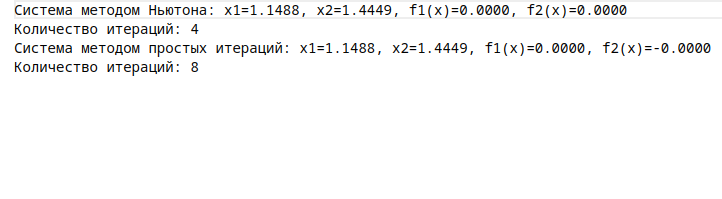
\includegraphics[width=.8\textwidth]{lab2.2}
\caption{Вывод в консоли}
\end{figure}


\subsection{Исходный код}
\lstinputlisting[title=\texttt{2-2.cpp}]{../stud/svoevolin/2-2.cpp}
\pagebreak